% Options for packages loaded elsewhere
\PassOptionsToPackage{unicode}{hyperref}
\PassOptionsToPackage{hyphens}{url}
%
\documentclass[
]{article}
\usepackage{amsmath,amssymb}
\usepackage{lmodern}
\usepackage{iftex}
\ifPDFTeX
  \usepackage[T1]{fontenc}
  \usepackage[utf8]{inputenc}
  \usepackage{textcomp} % provide euro and other symbols
\else % if luatex or xetex
  \usepackage{unicode-math}
  \defaultfontfeatures{Scale=MatchLowercase}
  \defaultfontfeatures[\rmfamily]{Ligatures=TeX,Scale=1}
\fi
% Use upquote if available, for straight quotes in verbatim environments
\IfFileExists{upquote.sty}{\usepackage{upquote}}{}
\IfFileExists{microtype.sty}{% use microtype if available
  \usepackage[]{microtype}
  \UseMicrotypeSet[protrusion]{basicmath} % disable protrusion for tt fonts
}{}
\makeatletter
\@ifundefined{KOMAClassName}{% if non-KOMA class
  \IfFileExists{parskip.sty}{%
    \usepackage{parskip}
  }{% else
    \setlength{\parindent}{0pt}
    \setlength{\parskip}{6pt plus 2pt minus 1pt}}
}{% if KOMA class
  \KOMAoptions{parskip=half}}
\makeatother
\usepackage{xcolor}
\usepackage[margin=1in]{geometry}
\usepackage{graphicx}
\makeatletter
\def\maxwidth{\ifdim\Gin@nat@width>\linewidth\linewidth\else\Gin@nat@width\fi}
\def\maxheight{\ifdim\Gin@nat@height>\textheight\textheight\else\Gin@nat@height\fi}
\makeatother
% Scale images if necessary, so that they will not overflow the page
% margins by default, and it is still possible to overwrite the defaults
% using explicit options in \includegraphics[width, height, ...]{}
\setkeys{Gin}{width=\maxwidth,height=\maxheight,keepaspectratio}
% Set default figure placement to htbp
\makeatletter
\def\fps@figure{htbp}
\makeatother
\setlength{\emergencystretch}{3em} % prevent overfull lines
\providecommand{\tightlist}{%
  \setlength{\itemsep}{0pt}\setlength{\parskip}{0pt}}
\setcounter{secnumdepth}{-\maxdimen} % remove section numbering
\usepackage{booktabs}
\usepackage{longtable}
\usepackage{array}
\usepackage{multirow}
\usepackage{wrapfig}
\usepackage{float}
\usepackage{colortbl}
\usepackage{pdflscape}
\usepackage{tabu}
\usepackage{threeparttable}
\usepackage{threeparttablex}
\usepackage[normalem]{ulem}
\usepackage{makecell}
\usepackage{xcolor}
\ifLuaTeX
  \usepackage{selnolig}  % disable illegal ligatures
\fi
\IfFileExists{bookmark.sty}{\usepackage{bookmark}}{\usepackage{hyperref}}
\IfFileExists{xurl.sty}{\usepackage{xurl}}{} % add URL line breaks if available
\urlstyle{same} % disable monospaced font for URLs
\hypersetup{
  pdftitle={Untitled},
  hidelinks,
  pdfcreator={LaTeX via pandoc}}

\title{Untitled}
\author{}
\date{\vspace{-2.5em}2022-10-27}

\begin{document}
\maketitle

\begin{verbatim}
## -- Attaching packages --------------------------------------- tidyverse 1.3.2 --
## v ggplot2 3.3.5     v purrr   0.3.4
## v tibble  3.1.6     v dplyr   1.0.8
## v tidyr   1.2.0     v stringr 1.4.0
## v readr   2.1.2     v forcats 0.5.1
## -- Conflicts ------------------------------------------ tidyverse_conflicts() --
## x dplyr::filter() masks stats::filter()
## x dplyr::lag()    masks stats::lag()
## 
## Attaching package: 'kableExtra'
## 
## 
## The following object is masked from 'package:dplyr':
## 
##     group_rows
## 
## 
## 
## Attaching package: 'gridExtra'
## 
## 
## The following object is masked from 'package:dplyr':
## 
##     combine
\end{verbatim}

\hypertarget{task-1}{%
\subsection{Task 1:}\label{task-1}}

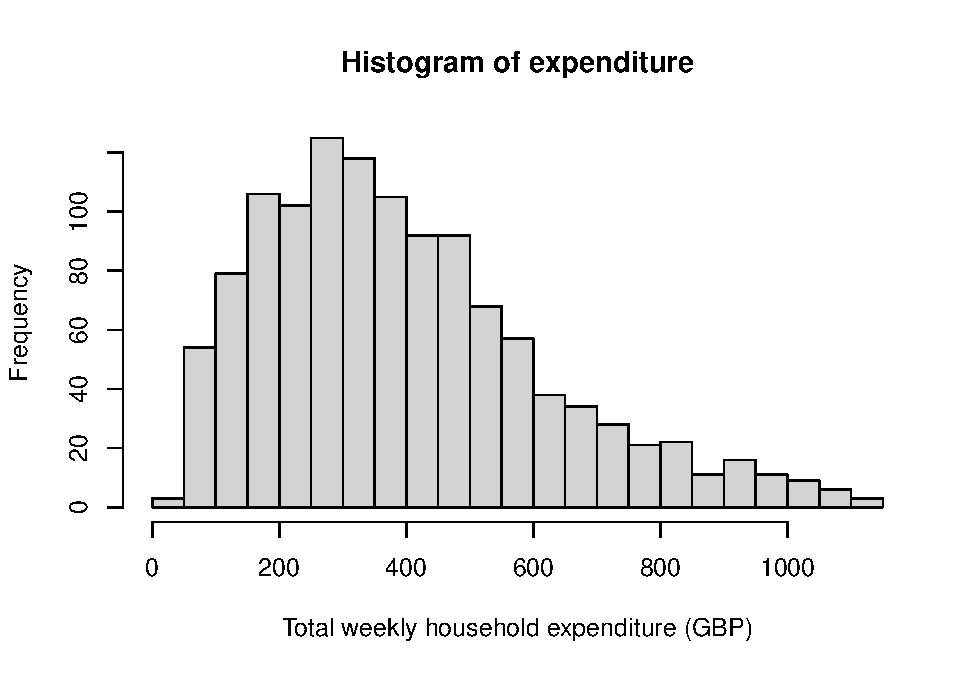
\includegraphics{Draft_1_files/figure-latex/unnamed-chunk-3-1.pdf}

\begin{verbatim}
## Warning: `guides(<scale> = FALSE)` is deprecated. Please use `guides(<scale> = "none")` instead.
## `guides(<scale> = FALSE)` is deprecated. Please use `guides(<scale> = "none")` instead.
## `guides(<scale> = FALSE)` is deprecated. Please use `guides(<scale> = "none")` instead.
## `guides(<scale> = FALSE)` is deprecated. Please use `guides(<scale> = "none")` instead.
## `guides(<scale> = FALSE)` is deprecated. Please use `guides(<scale> = "none")` instead.
\end{verbatim}

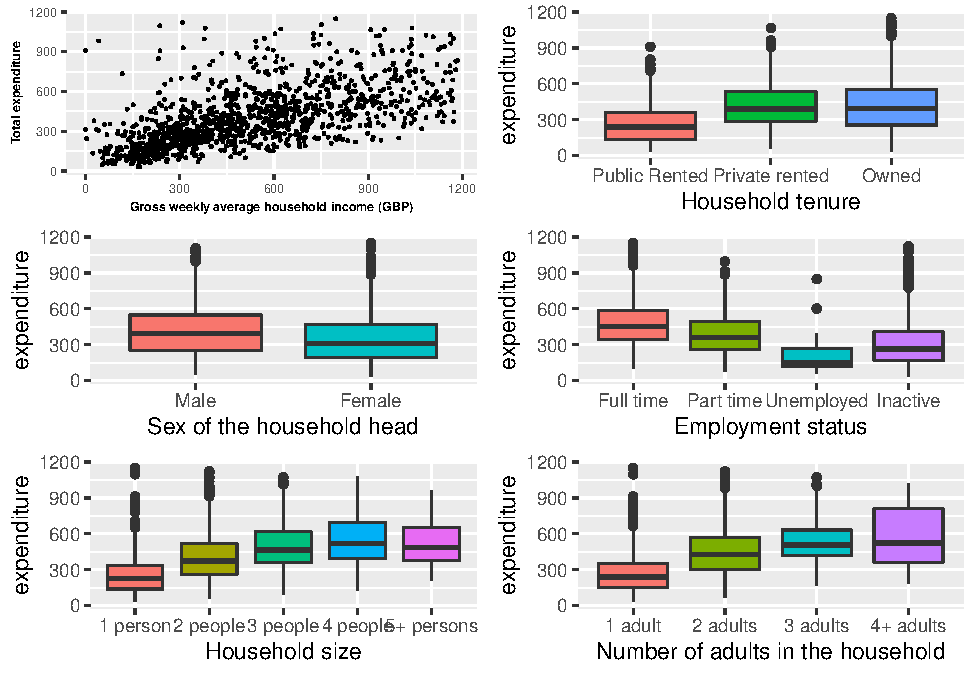
\includegraphics{Draft_1_files/figure-latex/unnamed-chunk-3-2.pdf}

Looking at the above histogram of expenditure it shows that expenditure
has a positively skewed distribution. Noticing this after applying a log
transform the histogram of log expenditure has a more normal looking
distribution.

Investigating covarits against expenditure we can see that there is a
positive association between household income and expenditure. Looking
at the various factor variables using box plots\ldots{}

\hypertarget{part-2}{%
\paragraph{Part 2:}\label{part-2}}

\begin{table}
\centering\begingroup\fontsize{15}{17}\selectfont

\begin{tabular}{l|r|r}
\hline
term & estimate & std.error\\
\hline
(Intercept) & 147.223766 & 10.3856098\\
\hline
income & 0.486028 & 0.0177632\\
\hline
\end{tabular}
\endgroup{}
\end{table}

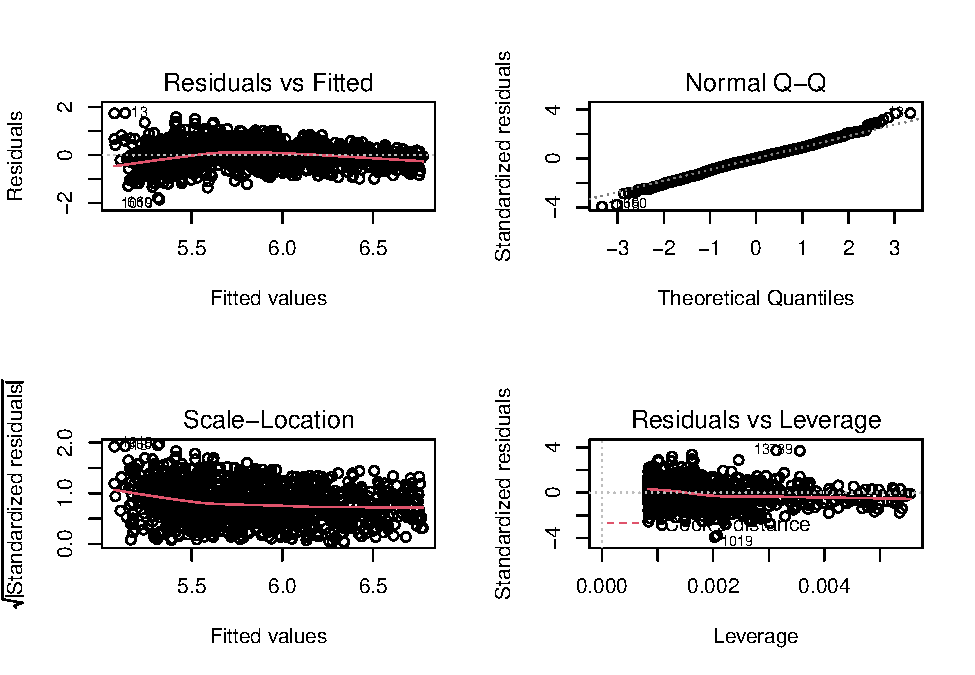
\includegraphics{Draft_1_files/figure-latex/unnamed-chunk-6-1.pdf}
Fitting a linear model \(y_{i}=\beta_{0}+\beta_{1}x_{i}+\epsilon\) with
the response \(y\) the expenditure,the explanatory variable \(x\) the
income and \(i \in \{1,...,1200\}\). The above table shows the estimated
values of the intercept (\(\beta_0\)) and the estimated `effect' of a 1
pound increase in income on expenditure \(\beta_1\) and there standard
errors.

Viewing the diagnostic plots for this model. The fitted vs residual plot
shows the residuals are not equally spread around 0 with a greater
spread of residuals above zero, meaning the assumption of linearity may
not hold. Furthermore, the QQ normal plot has a u shape with the tails
diverging heavily away from the straight line. This implies the
normality assumption is invalid.

\hypertarget{part-3}{%
\paragraph{Part 3:}\label{part-3}}

\begin{table}
\centering\begingroup\fontsize{15}{17}\selectfont

\begin{tabular}{l|r|r}
\hline
term & estimate & std.error\\
\hline
(Intercept) & 103.1753319 & 18.0506419\\
\hline
income & 0.6897522 & 0.0706466\\
\hline
I(income^2) & -0.0001761 & 0.0000591\\
\hline
\end{tabular}
\endgroup{}
\end{table}

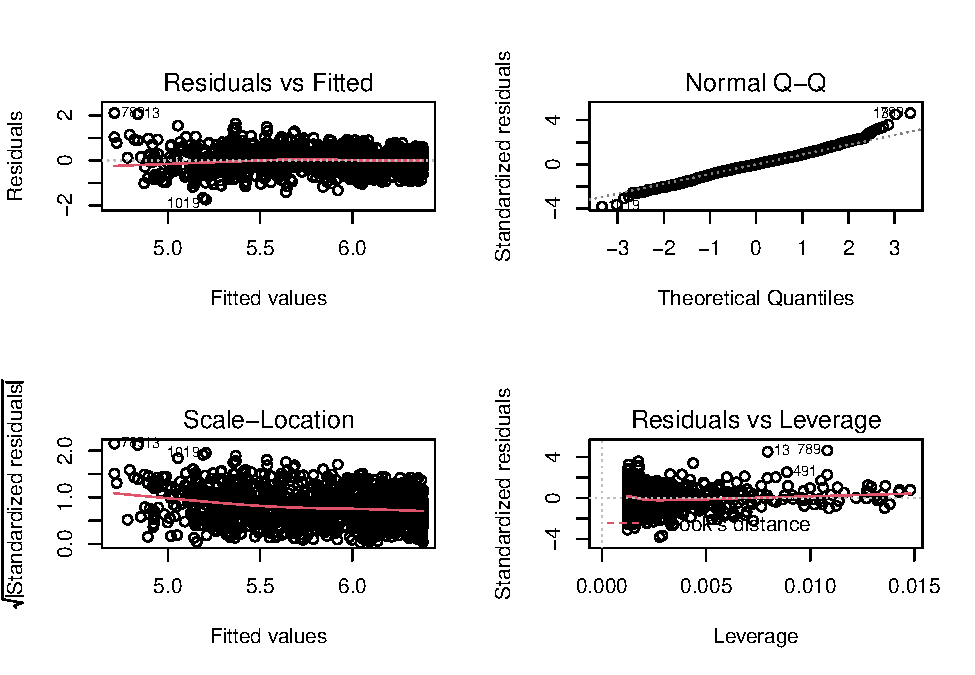
\includegraphics{Draft_1_files/figure-latex/unnamed-chunk-7-1.pdf}
Fitting a new linear model
\(y_{i}=\beta_{0}+\beta_{1}x_{i}+\beta_2x^2_{i}+\epsilon\) gives the
above estimated coefficients. Looking at the diagnostic plots, in the
fitted vs residual plot the residual values increase as the fitted
values increase thus the homoscedasticity assumption may not be valid.
The tails in the normal QQ plot also still deviate heavily away from the
straight line meaning the normality assumption is invalid.

\hypertarget{part-4}{%
\paragraph{Part 4:}\label{part-4}}

\begin{table}
\centering\begingroup\fontsize{15}{17}\selectfont

\begin{tabular}{l|r|r}
\hline
term & estimate & std.error\\
\hline
(Intercept) & 5.0739718 & 0.0281893\\
\hline
income & 0.0014356 & 0.0000482\\
\hline
\end{tabular}
\endgroup{}
\end{table}

\includegraphics{Draft_1_files/figure-latex/unnamed-chunk-8-1.pdf}
Fitting the model \(log(y_{i})=\beta_{0}+\beta_{1}x_{i}+\epsilon\). The
data appears to be hetroscedastic as the fitted vs residual plot points
spread decreases as fitted values increases/ not. The QQ plot shows the
residuals stay close to the straight line thus normality assumption is
valid.

\hypertarget{part-5}{%
\paragraph{Part 5:}\label{part-5}}

\begin{verbatim}
## 
## Call:
## lm(formula = log(expenditure) ~ income + I(income^2), data = expend.df)
## 
## Residuals:
##      Min       1Q   Median       3Q      Max 
## -1.73608 -0.26761 -0.00464  0.27537  2.10503 
## 
## Coefficients:
##               Estimate Std. Error t value Pr(>|t|)    
## (Intercept)  4.710e+00  4.747e-02  99.223   <2e-16 ***
## income       3.117e-03  1.858e-04  16.777   <2e-16 ***
## I(income^2) -1.453e-06  1.554e-07  -9.349   <2e-16 ***
## ---
## Signif. codes:  0 '***' 0.001 '**' 0.01 '*' 0.05 '.' 0.1 ' ' 1
## 
## Residual standard error: 0.4564 on 1197 degrees of freedom
## Multiple R-squared:  0.4644, Adjusted R-squared:  0.4635 
## F-statistic: 518.9 on 2 and 1197 DF,  p-value: < 2.2e-16
\end{verbatim}

\includegraphics{Draft_1_files/figure-latex/unnamed-chunk-9-1.pdf}

\(log(y_{i})=\beta_{0}+\beta_{1}x_{i}+\beta_{2}x^2_{i}+\epsilon\)

\end{document}
